\chapter{Implementarea aplicației mobile}
\thispagestyle{pagestyle}

În acest capitol este prezentat modul de implementare și funcționare al aplicației mobile ce comunică cu placa de dezvoltare Arduino Mega. Aplicația trebuie să se conecteze la modulul Bluetooth HC-05 legat la placa de dezvoltare, să citească datele oferite de senzori și să le afișeze în timp real.

Pentru dezvoltarea acestei aplicații am folosit mediul de programare Android Studio și este destinată dispozitivelor mobile ce folosesc sistemul de operare Android. Limbajul de programare folosit pentru implementarea aplicației este Java, Android Studio oferind un editor de cod performant pentru acesta. Totodată, acest mediu software oferă și un emulator care permite utilizatorilor să testeze aplicații Android pe un dispozitiv virtual.

Este folosită versiunea 34 de SDK (Softwear Development Kit) Android ceea ce inseamnă că aplicația este disponibilă pentru dispozitive ce ruelază sistemul de operare Android 14. De asemenea, versiunea minimă de SDK Android setată este 23, astfel orice dispoztiv ce ruleză cel puțin versiunea Androird 6.0 (Marshmallow \cite{marhsmallow}) poate folosi aplicația.

Primul pas în crearea aplicației a fost crearea unei interfețe intuitive ce este ușor de folosit pentru utilizator. Android Studio oferă un sistem de drag and drop, unde se poate alege dintr-o listă vastă de componente UI (User Interface) cum ar fi butoane, câmpuri de text, afișaj de imagine, pentru a fi folosite în interfața aplicației. Astfel, este folosit un buton pentru conectarea la modulul HC -05 și un câmp de text pentru afișarea datelor recepționate. Aspectul butonului, al câmpului de text, dar și al fundalului aplicației poate fi modificat folosind fișiere \texttt{.xml} în folderul \texttt{res} unde se găsesc toate elementele vizuale. Astfel, butonului i s-a aplicat un radient de culori, iar marginile i-au fost rotunjite. Câmpului de text i-a fost adăugată o margine de culoare diferită și de asemenea i s-au rotunjit marginile.

\begin{figure}[H]
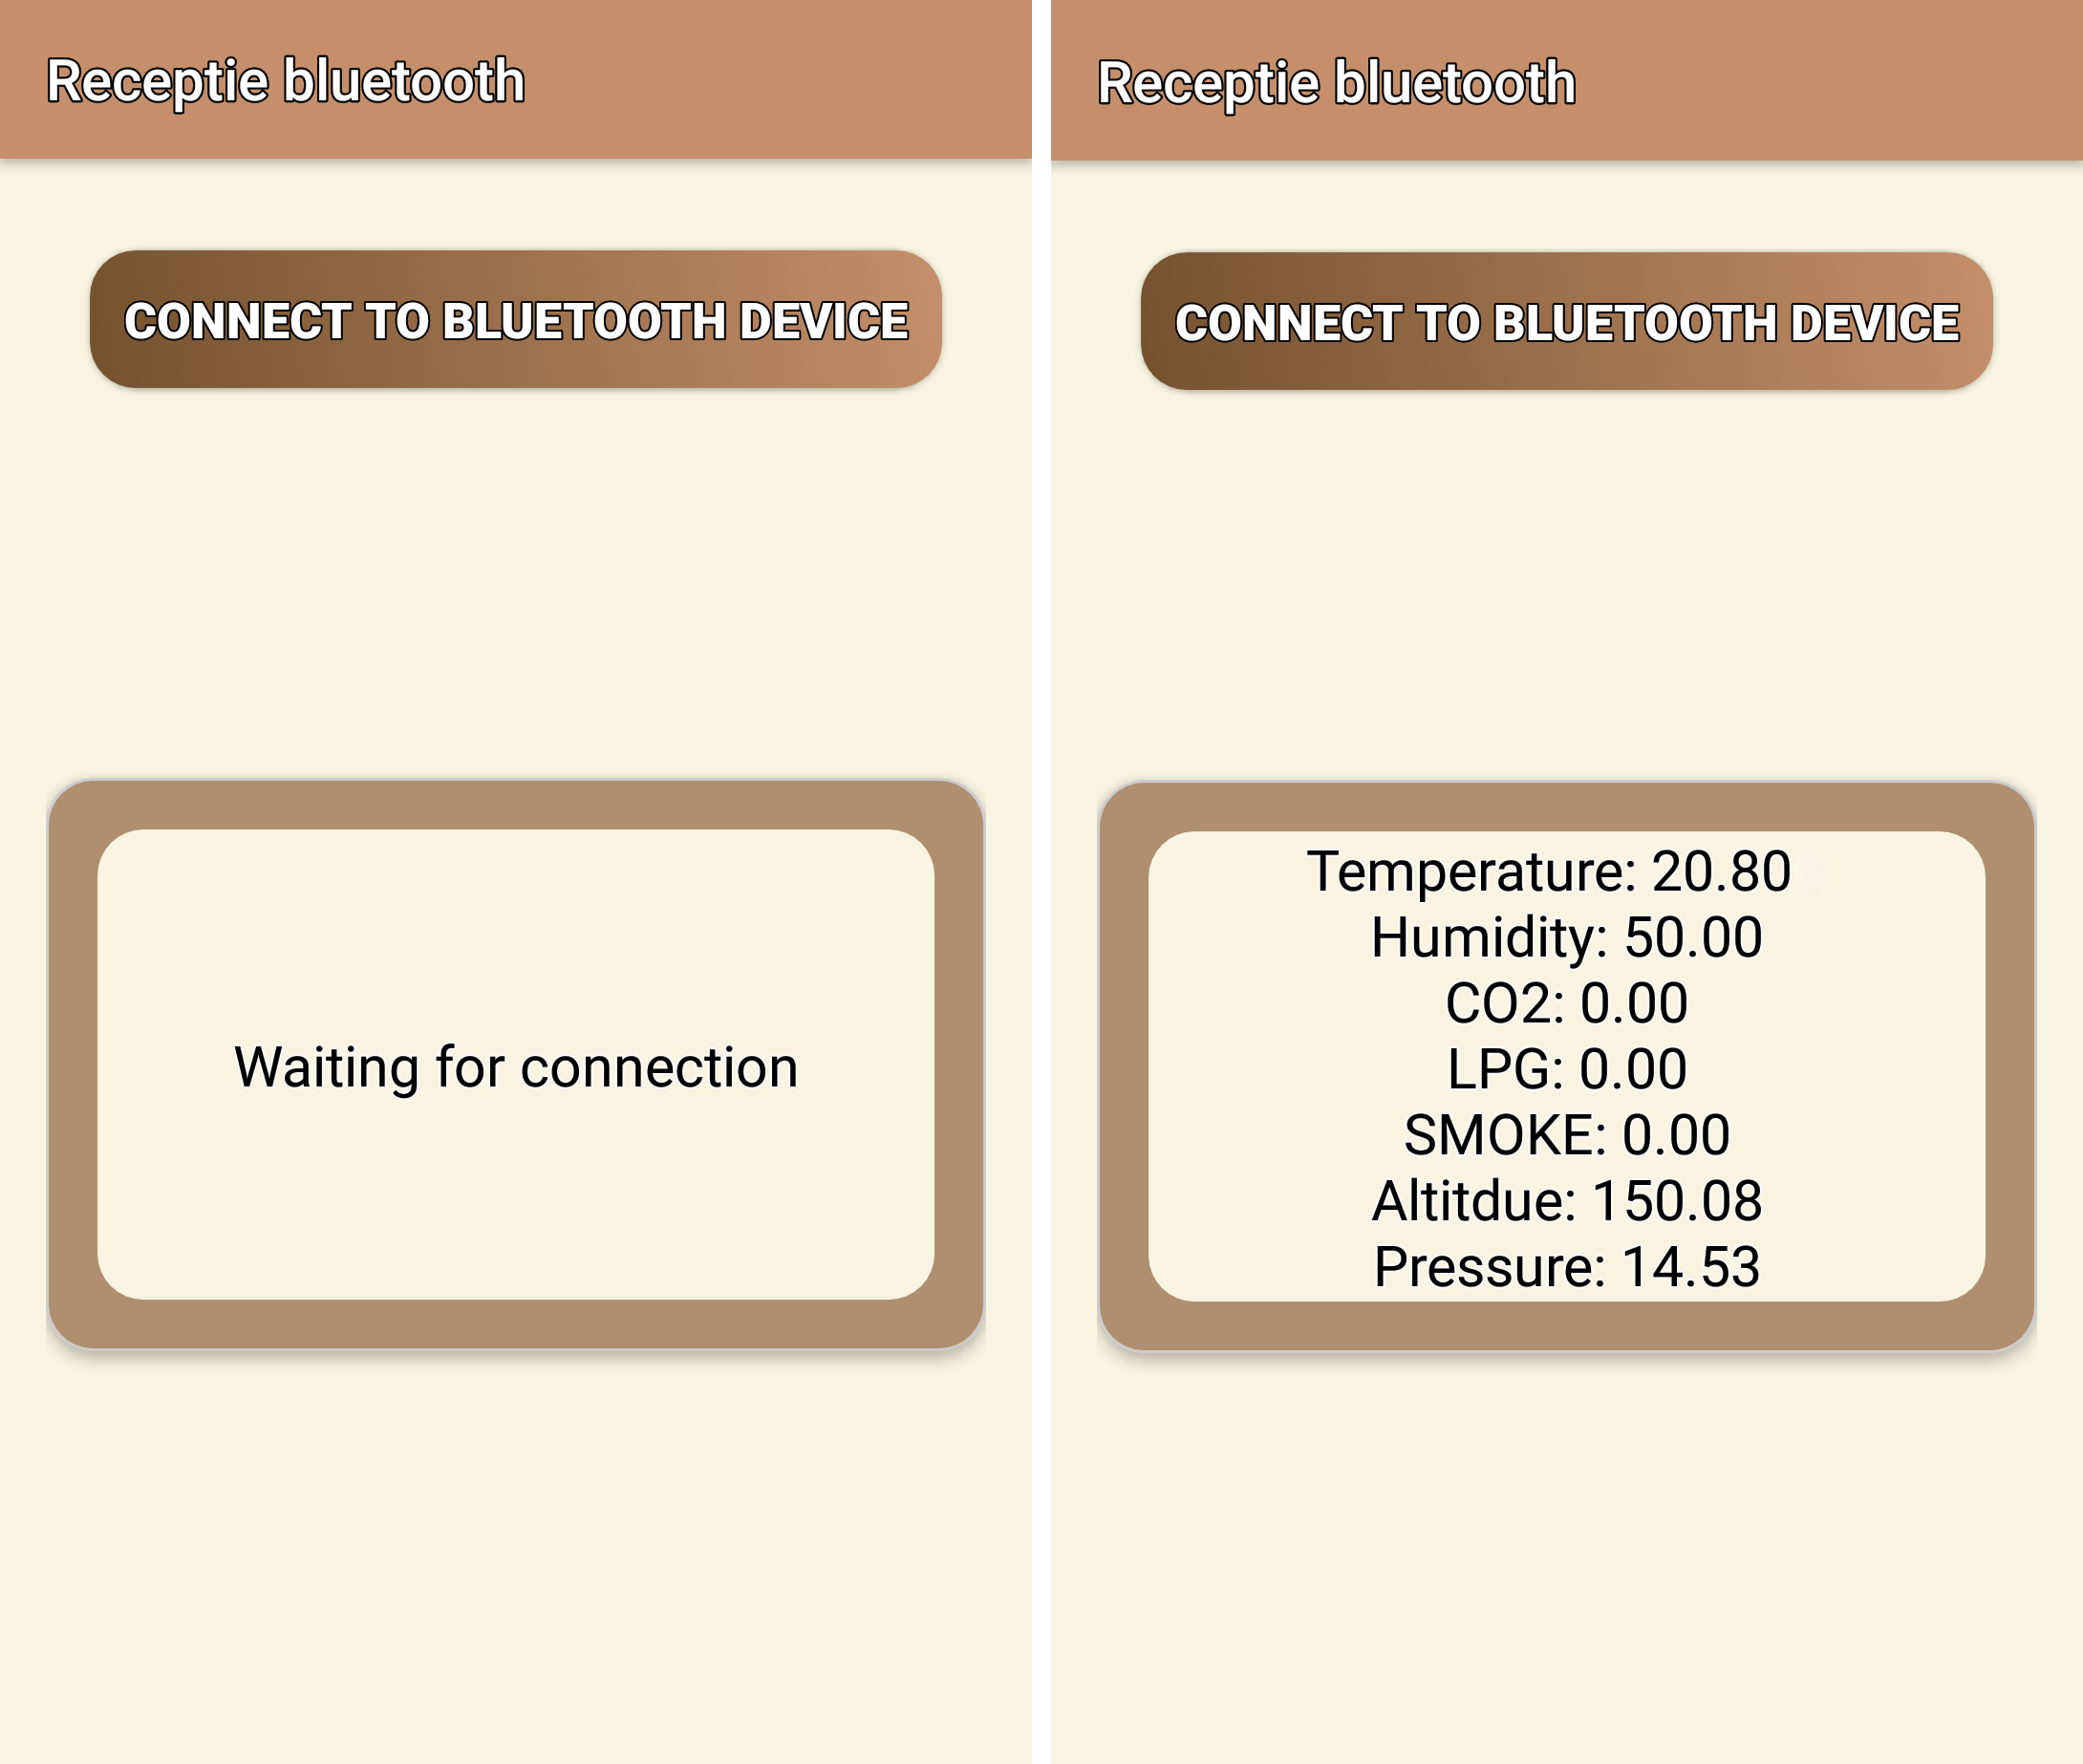
\includegraphics[width=0.6\linewidth]{bachelors_ro/images/bt_app_combined_separted.png}
\caption{Interfața aplicației înainte și după conectare}
\label{fig:bt_app_combined_separted}
\end{figure}

Următorul pas este implementarea codului de conexiune și citire a datelor trimise de modulul Bluetooth. Pentru ca aplicația să poată utiliza Bluetooth-ul este nevoie să ne folosim de API-ul (Application Programming Interface) Bluetooth ofeirt de Android \cite{bt_api}. În Fragmentul \ref{code:bt_api_classes} sunt prezentate clasele ce facilitează conexiunea la Bluetooth a aplicației și adresa MAC (media access control) a modulului. \texttt{deviceUUID} (Universally Unique Identifier) este folosit pentru a identifica tipul de serviciu Bluetooth. String-ul de la linia \textit{(6)} este folosit ca UUID și reprezintă serviciul SPP (Serial Port Profile).

\begin{code}[H]
\begin{lstlisting}[language=Java]
private BluetoothDevice bluetoothDevice;
private BluetoothAdapter bluetoothAdapter;
private BluetoothSocket bluetoothSocket;

private static final String deviceAddress = "**:**:**:**:**:**";
private static final UUID deviceUUID = UUID.fromString("00001101-0000-1000-8000-00805F9B34FB");

\end{lstlisting}
\caption{Clasele folosite din Bluetooth API \cite{bt_api}}
\label{code:bt_api_classes}
\end{code}

Chiar și cu toate datele de conectare oferite în Fragmentul \ref{code:bt_api_classes}, aplicația are nevoie de permisiuni de conectare la BLuetooth ce sunt oferite prin adăugarea Fragmentului \ref{code:bt_permisiuni} în fișierul \texttt{AndroidManifest.xml}.

\begin{code}[H]
\begin{lstlisting}[language=XML]
<uses-permission android:name="android.permission.BLUETOOTH_CONNECT" />
<uses-permission android:name="android.permission.BLUETOOTH"/>
<uses-permission android:name="android.permission.BLUETOOTH_ADMIN"/>
<uses-permission android:name="android.permission.BLUETOOTH_SCAN" />
\end{lstlisting}
\caption{Permisiunile de acces Bluetooth \cite{bt_perm}}
\label{code:bt_permisiuni}
\end{code}

Prima funcție ce trebuie apelată este funcția \texttt{onCreate()} ce inițializează aplicația. În interiorul acesteia avem funcția \texttt{setContentView(R.layout.activity\_main)} ce este apelată cu argumentul \texttt{R.layout.activity\_main} care inițalizează interfața definită anterior. Tot în corupul funcției \texttt{onCreate()} este inițializat și butonul ce conectează telefonul și modulul de Bluetooth. Asupra butonului este executată funcția \texttt{buttonConnect.setOnClickListener} pentru ca în momentul apăsării acesta să realizeze conexiunea cu modulul și să verifice permisiunile de conectare.

\begin{code}[H]
\begin{lstlisting}[language=Java]
private void connectToBluetoothDevice() {
    bluetoothDevice = bluetoothAdapter.getRemoteDevice(deviceAddress);
    try {
         bluetoothSocket = bluetoothDevice.createRfcommSocketToServiceRecord(deviceUUID);
         bluetoothSocket.connect();
        inputStream = bluetoothSocket.getInputStream();
         startReadingData();
    } catch (IOException e) {
        Log.e(TAG, "Error connecting", e);
    }
 }
\end{lstlisting}
\caption{Funcția de conectare la Bluetooth \cite{bt_api}}
\label{code:bt_conexiune}
\end{code}

În Fragmentul \ref{code:bt_conexiune} este prezentată funcția de conectare a dispozitiviului la Bluetooth. Inițial se obține referința către dispozitivul Bluetooth la care dorim să ne conectăm folosind metoda \texttt{bluetoothAdapter.getRemoteDevice(deviceAddress)} în care argumentul reprezintă adresa MAC a dispozitivului. Apoi, la linia \textit{(4)} se creează un socket RFCOMM (Serial Port Profile, iar metoda are ca argument \texttt{deviceUUID} pentru a identifica serviciul de conectare (SPP). După crearea socket-ului, se încearcă conectare cu dispozitivul. Dacă aceasta reușește să se stabilească, se deschide un flux de date, iar funcția \texttt{startReadingData()} este apleată pentru începerea citirii datelor. Dacă conectarea eșuează, se aruncă o excepție.

În Fragmentul \ref{code:bt_read_data} este prezentată metoda \texttt{readData()} ce citește datele primite de la placa de dezvoltare Arduino Mega. Pentru început, este nevoie de un flag \texttt{isReading} pentru a verifica dacă procesul de citire este activ, apoi este declarat obiectul de tip \texttt{Thread} care se ocupă de citirea propriu zisă. La liniile \textit{(4)} și \textit{(5)} avem variabila unde se va stoca șirul de caractere primit (\texttt{buffer}) și indexul acestuia. 

Cu ajutorul buclei \texttt{while(isReading)} menține execuția pornită atât timp cât se pot citi date. Apoi, se încearcă citire unui byte din inputStream, dacă citirea are succes se continuă procesarea datelor. Datele primite au un format special conceput astfel încât un set complet de date are ca terminator simbolul \texttt{\$}. Din acest motiv la linia \textit{(10)} se verifică dacă mesajul a fost transmis în întregime. În cazul în care mesajul este complet, acesta se stochează într-un șir de caractere, indexul buffer-ului se setează pe 0, iar folosind un \texttt{handler} se actualizează câmpul de text pentru a afișa datele primite. \texttt{Thread.sleep(1000)} este folosit pentru a citi datele o dată la o secundă. 


\begin{code}[H]
\begin{lstlisting}[language=Java]
private void readData() {
  isReading = true;
  readThread = new Thread(() -> {
    final byte[] buffer = new byte[1024];
    int bufferPosition = 0;

    while (isReading) {
      try {
        if (inputStream.read(buffer, bufferPosition, 1) > 0) {
          if (buffer[bufferPosition] == '$') {
            final String readMessage = new String(buffer, 0, bufferPosition).trim();
            bufferPosition = 0;
            handler.post(() -> textViewData.setText(readMessage));
            Thread.sleep(1000);
          } else {
            bufferPosition++;
          }
        }
      } catch (IOException | InterruptedException e) {
        Log.e(TAG, "Error reading data", e);
        isReading = false;
      }
    }
  });
  readThread.start();
}
\end{lstlisting}
\caption{Funcția de conectare la Bluetooth \cite{bt_transfer}}
\label{code:bt_read_data}
\end{code}

În final, funcția \texttt{onDestroy()} va asigura închiderea conexiunii și thread-ul de citire este oprit la închiderea aplicației.

Astfel, aplicația a fost creată și poate rula pe orice dispozitiv ce utilizează minim versiunea 6.0 de Android. Rezultatul final este prezent în Figura \ref{fig:bt_app_combined_separted}.

